%KECReportFormat.tex
%%%%%%%%%%%%%%%%%%%%%%%%%%%%%%%%%%%%%%%%%%%%%%%%%%%%%%%%%%%%%%%%%%%%%%%%%%%
%DO NOT MAKE CHANGES IN THIS FILE

\documentclass[12pt, a4paper]{report}
\usepackage[left = 1.5in, right = 1in, top = 1in, bottom = 1in]{geometry}%for margin
\usepackage{amsfonts, amsmath, amssymb} %for mathematical equations
\usepackage{graphicx} %for images
\usepackage{times} %font Times New Roman Font
\usepackage{float} %required if you use H(strictly here) position for floats
\usepackage[skip = 8pt,tableposition=top, figureposition=bottom]{caption}%adjust spacing of captions and specify where captions are
\usepackage{hyperref} % for easy Navigation in document, also puts links in TOC, LOF, LOT...
\usepackage{setspace} %to change line spacing in some portion \singlespacing \onehalfspacing \doublespacing
\usepackage{acro} %for List of Abbrreviation and Symbol
\acsetup{first-style = short} % set to display only short form on the command \ac{}

%packages required for complex tables
\usepackage{bigstrut} 
\usepackage{multirow}

\renewcommand{\contentsname}{Table of Contents} %Change TOC Heading ... default is "Contents" 

\parindent 0pt	%removes the indent in paragraph
\setlength{\parskip}{18pt}	%for paragraph spacing
\renewcommand{\baselinestretch}{1.5}   %Line Spacing = 1.5 line-spaces

%to reduce spacing in sections
\usepackage{titlesec}
\titlespacing*{\section}{0pt}{0pt}{0pt} %left, top, bottom spacings
\titlespacing*{\subsection}{0pt}{0pt}{0pt}
\titlespacing*{\subsubsection}{0pt}{0pt}{0pt}
\titlespacing*{\paragraph}{0pt}{0pt}{0pt}
\titlespacing*{\subparagraph}{0pt}{0pt}{0pt}

%adjust fontsizes\ of sections
\titleformat*{\section}{\fontsize{14pt}{18pt}\bfseries}
\titleformat*{\subsection}{\fontsize{13pt}{18pt}\bfseries}
\titleformat*{\subsubsection}{\fontsize{12pt}{18pt}\bfseries}
\titleformat*{\paragraph}{\fontsize{12pt}{18pt}\bfseries}
\titleformat*{\subparagraph}{\fontsize{12pt}{18pt}\bfseries}

%to reduce separation between points in list
\usepackage{enumitem}
\setlist[enumerate]{nosep} % no separation between items in enumerate
\setlist[itemize]{nosep} % no separation between items in itemize
%use \vspace{-18pt} before list to reduce paragraph spacing between list and preceeding paragraph.

%Changes for Chapter Heading Spacing and formats for numbered chapters
\makeatletter
\def\@makechapterhead#1{%
  %\vspace*{50pt}%
  {  \MakeUppercase{\ifnum \c@secnumdepth >\m@ne
        \fontsize{16pt}{1}\bfseries \@chapapp \space \thechapter\vspace{5pt}\\
    \fi
    \interlinepenalty\@M
     \bfseries #1}\par\nobreak
    %\vskip 0pt
  }}
\makeatother

%%%%%%%%%%%%%%%%%%%%%%%%%%%%%%%%%%%%%%%%%%%%%%%%%%%%%%%%%%%
%to adjust Heading spacings and fonts For unnumbered chapters, TOC, LOF ...
\makeatletter
% Redefine the \chapter* header macro to remove vertical space
\def\@makeschapterhead#1{%
  %\vspace*{50\p@}% Remove the vertical space
  {\newpage \parindent \z@ \raggedright
    \normalfont
    \interlinepenalty\@M
    \center \fontsize{16pt}{1} \bfseries \MakeUppercase{#1}\par\nobreak
    %\vskip 18\p@ % adjust space after heading 18pt
  }}
\makeatother 
%%%%%%%%%%%%%%%%%%%%%%%%%%%%%%%%%%%%%%%%%%%%%%%%%%%%%%%%%%%

%%%%%%%%%%%%%%%%%%%%%%%%%%%%%%%%%%%%%%%%%%%%%%%%%%%%%%%%%%%%%%%%%%%%%%%%%%%
% newcommand for generating Cover Page
\newcommand{\KECcoverpage}
{
\begin{titlepage}
\begin{center}
\Large{\textbf{KANTIPUR ENGINEERING COLLEGE}}\\
\large{\textbf{(Affiliated to Tribhuvan University)}}\\
\large{\textbf{Dhapakhel, Lalitpur}}\\
\vfill	%vertically fill the space 
\begin{figure}[h] % h: put logo "here"
\begin{center}

\includegraphics[width=25mm, height = 25mm]{images/logo.png}
\end{center}
\end{figure}

\large{\textbf{[Subject Code: \subCode]}}\\ %Change This Line
\large{\textbf{A \MakeUppercase{\project} \MakeUppercase{\doc} ON}}\\ %Change This Line
\Large{\textbf{\MakeUppercase{\projectTitle}}}\\

\vfill	%vertically fill the space 
\large{\textbf{Submitted by:}}\\
\large{\textbf{\submittedBy}}\\
\vfill	%vertically fill the space 
\textbf{A \MakeUppercase{\project} SUBMITTED IN PARTIAL FULFILLMENT OF THE REQUIREMENT FOR THE DEGREE OF \MakeUppercase{\degree}}\\

\vfill	%vertically fill the space 
\large{\textbf{Submitted to:}}\\
\large{\textbf{\submittedTo}}\\
\vfill
\large{\textbf{\defMonth, \defYear}}
\pagebreak
\end{center}
\end{titlepage}
}
%%%%%%%%%%%%%%%%%%%%%%%%%%%%%%%%%%%%%%%%%%%%%%%%%%%%%%%%%%%%%%%%%%%%%%%
% newcommand for generating Cover Page
%Title Page
\newcommand{\KECtitlepage}
{
\begin{titlepage}
\begin{center}
\Large{\textbf{\MakeUppercase{\projectTitle}}}\\

\vfill	%vertically fill the space 

\large{\textbf{Submitted by:}}\\
\large{\textbf{\submittedBy}}\\


\ifhassupervisor % Displays Supervisor name only if \hassupervisortrue
	\vfill	%vertically fill the space 
	\large{\textbf{Supervised by:}}\\
	\large{\textbf{\supervisor}}\\
	\large{\textbf{\degSup}}\\
\fi

\vfill	%vertically fill the space 
\textbf{A \MakeUppercase{\project} SUBMITTED IN PARTIAL FULFILLMENT OF THE REQUIREMENT FOR THE DEGREE OF \MakeUppercase{\degree}}\\

\vfill	%vertically fill the space 
\large{\textbf{Submitted to:}}\\
\large{\textbf{\submittedTo}}\\
\large{\textbf{Kantipur Engineering College}}\\
\large{\textbf{Dhapakhel, Lalitpur}}\\

\vfill
\large{\textbf{\defMonth, \defYear}}
\thispagestyle{empty}\\ %to remove page number
\pagebreak
\end{center}
\end{titlepage}
}
%%%%%%%%%%%%%%%%%%%%%%%%%%%%%%%%%%%%%%%%%%%%%%%%%%%%%%%%%%%%%%%%%%%%%%
%command for copyright page
\newcommand{\KECcopyright}
{
\chapter*{Copyright}%Required only for Final Defense of Major Project
\addcontentsline{toc}{chapter}{Copyright}
The author has agreed that the library, Kantipur Engineering Collage, may make this report freely available for inspection. Moreover the author has agreed that permission for extensive copying of this report for scholarly purpose may be granted by the supervisor(s), who supervised the project work recorded herein or, in their absence, by the Head of the Department wherein this project was done. It is understood that due recognition will be given to the author of this report and to the \submittedTo, Kantipur Engineering College in any use of the material of this report. Copying or publication or other use of this report for financial gain without approval of the \submittedTo, Kantipur Engineering College and author’s written permission is prohibited.\par Request for permission to copy or to make any other use of the material in this report in whole or in part should be addressed to:

Head\\
\submittedTo\\
Kantipur Engineering College\\
Dhapakhel, Lalitpur\\
Nepal
}
%%%%%%%%%%%%%%%%%%%%%%%%%%%%%%%%%%%%%%%%%%%%%%%%%%%%%%%%%%%%%%%%%%%%%%
%command for Approval Letter
\newcommand{\KECapproval}
{
\chapter*{Kantipur Engineering College
\vskip -10pt}%Required only for Final Defense of Major Project
\begin{center}
\fontsize{12.8pt}{1} %size decreaced to adjust department name in single line
\textbf{
\MakeUppercase{\submittedTo}\\ %for department name
}
\vskip 10pt
\fontsize{16pt}{1}
\textbf{APPROVAL LETTER}
\end{center}
\vskip -16pt
\addcontentsline{toc}{chapter}{Approval Letter}%
The undersigned certify that they have read and recommended to the Institute of Engineering for acceptance, a project report entitled "\projectTitle " submitted by \\
\submittedBy \\
in partial fulfillment for the degree of \degree. \par
{\vspace{25pt}
..........................................\\
Supervisor\\
\supervisor \\
\degSup\\
\vspace{25pt}\\
..........................................\\
External Examiner\\
\external\\
\degExternal\\
\vspace{25pt}\\
..........................................\\
\hod\\
Head of Department\\
\submittedTo
\vspace{10pt}\\
Date: \defMonth\space\defDay ,\space \defYear
\singlespacing\par
} %single spacing for the texts inside {}
}

%command for list of abbreviations
\newcommand{\KECloa}
{
\chapter*{List of Abbreviations}
\addcontentsline{toc}{chapter}{List of Abbreviations}
\vskip -42pt % to reduce space due to invisivle acronym class name
{
\singlespacing
\printacronyms[include-classes=abbr, name= ]
}

}

%command for list of symbols
\newcommand{\KEClos}
{
\chapter*{List of Symbols}
\addcontentsline{toc}{chapter}{List of Symbols}
\vskip -42pt % to reduce space due to invisivle acronym class name{
{
\singlespacing
\printacronyms[include-classes=symbol, name= ]
}
}

%command to adjust toc, lof, lot spacing
\newcommand{\KECadjusttocspacings}
{
\parskip 0pt % to remove paragraph spacing in TOC, LOF ...
\renewcommand{\baselinestretch}{0.1} % to adjust line spacing in toc
\newcommand*{\noaddvspace}{\renewcommand*{\addvspace}[1]{}}
\addtocontents{lof}{\protect\noaddvspace} %remove extra vertical space in LOF
\addtocontents{lot}{\protect\noaddvspace} %remove extra vertical space in LOT
} %includes the file KecReportFormat.tex that include all necessary formattings
%%%%%%%%%%%%%%%%%%%%%%%%%%%%%%%%%%%%%%%%%%%%%%%%%%%%%%%%%%%%%%%%%%%%%%%%%%%
%Define Macros for Details of your Project
\newcommand{\project}{Major Project} %Specify "Major Project" or "Minor Project"
\newcommand{\projectTitle}{Stock Price Prediction} %specify "Title" of Your Project
\newcommand{\doc}{Proposal} % specify the document you are preparing eg. "Proposal", "Mid-Term Report" or "Final Report" 
% Note that You have to sibmit "Final Report" for Pre-final defense as well.
\newcommand{\subCode}{CT755} %specify Subject of Your Project
\newcommand{\degree}{Bachelor in Computer Engineering} %specify your degree
\newcommand{\submittedBy}%Specify Names and Roll/Symbol Numbers of the Project Group Members
{
%Edit Member Names and Roll/Symbol No. and adjust width (\makebox[width]) if necessary 
\makebox[6cm]{Aman Devkota  \hfill[28808]}\\
\makebox[6cm]{Ankur Karmacharya  \hfill[28811]}\\
\makebox[6cm]{Prashad Adhikary  \hfill[28852]}
%\makebox[9cm]{Member Name \hfill [Roll/Symbol No.]}\\
} % Note that You must write your "Symbol Numbers"(Exam Roll Numbers) for Final Defenses

\newcommand{\submittedTo}{Department of Computer and Electronics Engineering} %specify your department
\newcommand{\hod}{Er. Rabindra Khati} %specify Head ot the department
\newcommand{\defYear}{2023} %Defense Year
\newcommand{\defMonth}{June} %Defense Month- January, February, ...
\newcommand{\defDay}{18} %specify Defense Day- 1, 2, ...

\newif\ifhassupervisor
\hassupervisorfalse % to display supervisor name use command- \hassupervisortrue
\newcommand{\supervisor}{none} % Specify Name of Supervisor for Major Project (write "none" if no Supervisor is assigned)
\newcommand{\degSup}{Supervisor's Designation\\Second Line of Designation (if required)} %Specify Designation of Supervisor for Major Project, use multiple lines (\\) if necessary
\newcommand{\external}{External's Name} %Specify Name of External for Major Project (Required for Black Book)
\newcommand{\degExternal}{External's Designation\\Second Line of Designation (if required)} %Specify Name of External for Major Project (Required for Black Book) , use multiple lines (\\) if necessary
%%%%%%%%%%%%%%%%%%%%%%%%%%%%%%%%%%%%%%%%%%%%%%%%%%%%%%%%%%%%%%%%%%%%%%%%%%%

%%%%%%%%%%%%%%%%%%%%%%%%%%%%%%%%%%%%%%%%%%%%%%%%%%%%%%%%%%%%%%%%%%%%%%%%%%%

%%%%%%%%%%%%%%%%%%%%%%%%%%%%%%%%%%%%%%%%%%%%%%%%%%%%%%%%%%%%%%%%%%%%%%%%%%%%%%%%%%%%%%%%%%%%%%%%%%%%

%%%%%%%%%%%%%%%%%%%%%%%%%%%%%%%%%%%%%%%%%%%%%%%%%%%%%%%%%%%%%%%%%%%%%%%%%%
%The Document
\setcounter{tocdepth}{3}
\setcounter{secnumdepth}{3}
\begin{document}

\KECcoverpage  
\KECtitlepage
\pagenumbering{roman} % starts pagenumberins in Roman numerals i, ii, ...

%Copyright Page is required for FINAL REPORT only. Comment this section for other Reports.
%\KECcopyright % defined in KECReportFormat.tex

%Approval Page is required for FINAL(Black Book Binded) REPORT of MAJOR PROJECT only. Comment this section for other Reports. 
%\KECapproval % defined in KECReportFormat.tex

\chapter*{Abstract} % The summary of your report
\addcontentsline{toc}{chapter}{Abstract}%to include this chapter in TOC 
Stock market prediction is when people try to figure out what the value of a stock will be in the future. They do this to make money by buying and selling stocks at the right time. Deep learning models are used to help predict stock prices. Recurrent neural networks are a type of deep learning model that is often used. There are different types of deep learning models that can be used depending on the situation. Predicting stock prices is difficult because there are many factors that can affect them. These factors can include things like politics, global economic conditions, and a company's financial performance. This project performs a comparative analysis of three deep learning models-the Long Short-term Memory (LSTM), Gated Recurrent Unit (GRU), and Vanilla RNN (VRNN)- in predicting the next day’s closing price of the Nepal Stock Exchange (NEPSE) index. The performances of employed models are compared using the standard assessment metrics-Root Mean Square Error (RMSE), Mean Absolute Percentage Error (MAPE), and Correlation Coefficient (R).
\par
\textbf{\textit{Keywords$-$}} \emph{LSTM, GRU, VRNN, NEPSE, Deep learning}

\chapter*{Acknowledgment}
\addcontentsline{toc}{chapter}{Acknowledgment}%to include this chapter in TOC
We would like to express sincere gratitude to Department head Er. Rabindra Khati, Project Co-ordinator Er. Bishal Thapa and all the faculty members of Kantipur Engineering College for the continuous support during this project for their patience, motivation,enthusiasm, and immense knowledge. Their guidance helped us in all time of research, development and implementation of this project.   \par
%Finally we would like to thank our family and friends for all the support and encouragement.\par
%to display members name under Acknowledgement
\begin{flushright}
\vskip -20pt
\setstretch{1.2}
\submittedBy

\end{flushright}

%to adjust spacings for TOC, LOF, LOT
{
%%%%%%%%%%%%%%%%%%%%%%%%%%%%%%%%%%%%%%%%%%%%%%%%%%%%%%%%%%%%%%%%%%%%%%%%%%%
%TOC, LOF and LOT
\KECadjusttocspacings % defined in KECReportFormat.tex to adjust spacings
\makeatletter
% to add vskip of 18 point which is reduced when parskip is set to 0 in \LECadjustspacings
\def\@makeschapterhead#1{%
  %\vspace*{50\p@}% Remove the vertical space
  {\newpage \parindent \z@ \raggedright
    \normalfont
    \interlinepenalty\@M
    \center \fontsize{16pt}{1} \bfseries \MakeUppercase{#1}\par\nobreak
   % \vskip 18\p@ % adjust space after heading 18pt
  }}
\makeatother 

\tableofcontents % prints table of contents
\listoffigures % prints list of figures
\addcontentsline{toc}{chapter}{List of Figures}
%\listoftables % prints list of table
%\addcontentsline{toc}{chapter}{List of Tables}
}
%%%%%%%%%%%%%%%%%%%%%%%%%%%%%%%%%%%%%%%%%%%%%%%%%%%%%%%%%%%%%%%%%%%%%%%%%%%

%comment this chapter if you don't have List of Abbreviations
%\KECloa % defined in KECReportFormat

%comment this chapter if you don't have List of Symbols
%\KEClos % defined in KECReportFormat

\newpage
\pagenumbering{arabic} % starts pagenumbering in arabic numerals

\chapter{Introduction}
\vspace{-18pt}
\section{Background}\label{sec:bkgrnd}%label your section if you require to refer them somewhere else in your document.
\vspace{-18pt}
The stock price is determined by the highest price a buyer is willing to pay or the lowest price a seller is willing to accept. Supply and demand are key factors that can affect stock prices. High demand can lead to an increase in stock price, while high supply can lead to a decrease. However, it is difficult to determine the exact factors that contribute to changes in demand and supply. Stock market prediction involves forecasting the future value of a stock. Financial analysts use two main schools of thought for analyzing and predicting stock markets: technical analysis and fundamental analysis. \cite{}%subarna
\par
 Machine learning models can learn a function by analyzing data without explicit programming. The performance of these algorithms depends on the representation of the data. However, stock market time-series data is difficult to map and is best described as a random walk, making feature engineering and prediction challenging. Therefore, deep learning models are the best available tool for stock market prediction.\cite{}%purano
 \par
 There are two schools of thought in developing predictive models for estimating stock prices. Classical thinking uses historical facts and indicators to predict future stock prices, often through variations of Autoregressive Integrated Moving Average (ARIMA) models. However, these statistical models may not efficiently capture the noisy and nonlinear behavior of stock market data. Modern theory assumes that historical data cannot reflect the exact upcoming structure due to inherent non-linearity in stock market data. With the rapid advancement of artificial intelligence and machine learning techniques, availability of large-scale data, and increased computational capabilities, robust machine learning models can capture nonlinear behavior and predict stock prices.\cite{}%meetwala

\section{Problem Statement}
\vspace{-18pt}
The stock market is a frequent topic in the media, with news outlets reporting on its daily fluctuations. Whenever the market experiences a new peak or dip, it garners significant attention. Developing an effective algorithm to forecast short-term stock prices could potentially boost investment rates and create more business prospects in the market.

\section{Objectives}
\vspace{-18pt}
The primary objectives of this projects are as follows:
\vspace{-18pt}
\begin{enumerate}[label=\roman*.]
\item Gathering the multifaceted information of NEPSE index, putting them together into a common framework, and constructing a reliable model for accurate predictions.
\item Conducting extensive data driven experimentation using customized parameters of LSTM, GRU, and VRNN models.
\item Performing comparative study of deep learning models (LSTM, GRU, and VRNN) for the best fit and forecasting under the identical conditions.
\item Conducting statistical experiment to validate and verify the reliability and robustness of the model.
\end{enumerate}
\section{Project Features}
\vspace{-18pt}
The project will be able to accomplish following:
\vspace{-18pt}
\begin{itemize}
\item Reliable
\item Accurate
\item User friendly
\item Efficient 
\end{itemize}
\section{Application Scope}
\vspace{-18pt}
Stock price prediction has various applications such as investment decision-making, risk management, algorithmic trading, portfolio optimization, and economic forecasting. Predicting stock prices can help investors make informed decisions, manage risk, optimize portfolios, and provide insights into the economy. It is a valuable tool for investors, financial institutions, and economists seeking to make informed decisions and manage risk.
\section{System Requirement}
\vspace{-18pt}
\subsection{Development Requirements}
\vspace{-18pt}
\subsubsection{Software Requirements}
\vspace{-10pt}
\begin{itemize}
\item Windows/Linux/Mac
\item HTML/CSS/JS
\item Jupyter Notebook
\item Python IDE
\end{itemize}
\subsubsection{Hardware Requirements}
\vspace{-10pt}
\begin{itemize}
\item PC with at least 4-8 GB RAM
\item  Higher graphics of at least 2 GB
\end{itemize}
\subsection{Deployment Requirements}
\vspace{-18pt}
\subsubsection{Software Requirements}
\vspace{-10pt}
\begin{itemize}
\item Web browser
\item Visual studio code
\item Pycharm
\end{itemize}
\vspace{-10pt}
\subsubsection{Hardware Requirements}
\vspace{-10pt}
\begin{itemize}
\item More than 1.5 GHz clock speed
\item Minimum 4 GB RAM
\end{itemize}
\label{tblSampleTable}
%\end{table}
\section{Project Feasibility}
\vspace{-18pt}
\subsection{Technical Feasibility}
\vspace{-18pt}
The technical feasibility assessment is focused on gaining in understanding of the present technical resources required by the system and their applicability to the expected needs of the proposed system. Regarding the proposed system, the technical requirement includes a PC.
\vspace{-18pt}
\subsection{Operational Feasibility}
\vspace{-18pt}
The user will not need any formal knowledge about programming so our project is operationally feasible.
\vspace{-18pt}
\subsection{Economic Feasibility}
\vspace{-18pt}
The purpose of the economic feasibility assessment is to determine the positive economic benefits to the user that the proposed system will provide. Most of the software used for the development is free. Thus, the project is economically feasible.
\vspace{-18pt}
\subsection{Schedule Feasibility}
\vspace{-18pt}
%\begin{figure}[!h] % tbh means top, bottom or here (priority: left to right)
%\begin{center}
	%
\includegraphics[width = 3in]{images/logo.png}
	%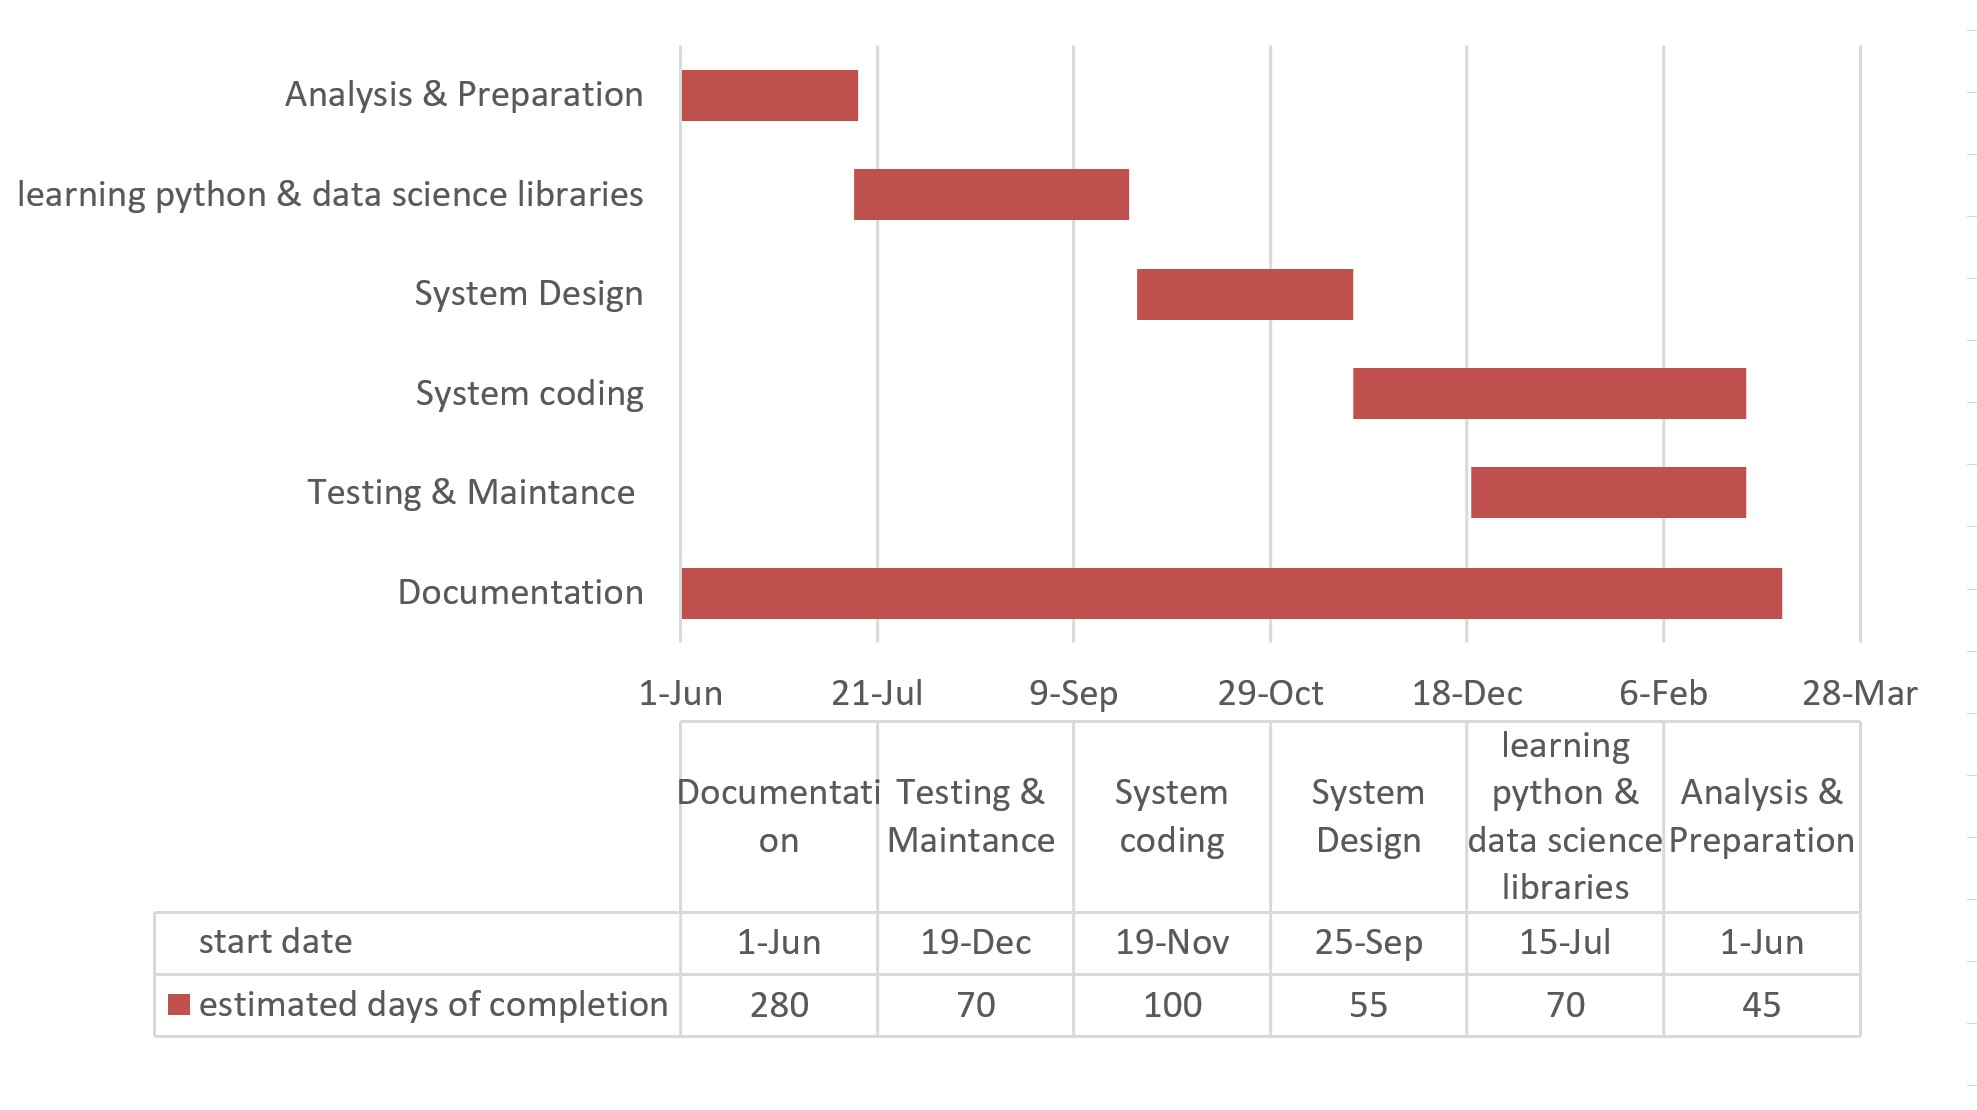
\includegraphics[width=6in]{Screenshot 2023-03-23 005901.jpg} 
	%\caption{Gantt Chart} %figure name
	%\label{figGanttChart} % for referencing
%\end{center}
%\end{figure}
\chapter{Literature Review}
\vspace{-18pt}
\section{Related Projects}
\vspace{-18pt}
\subsection{Zillow}
\vspace{-18pt}
 Zillow is a popular online real estate marketplace that provides an automated valuation model called the Zestimate. This model uses a combination of data from public records, user-submitted data, and machine learning algorithms to predict the value of a home.
 \vspace{-10pt}
\subsection{Redfin's Home Value Estimator}
\vspace{-18pt}
Redfin is another online real estate marketplace that provides a home value estimator tool that uses machine learning algorithms to predict the value of a home based on its location, features, and recent sales in the area.
\vspace{-10pt}
\subsection{House Canary}
\vspace{-18pt}
HouseCanary is a real estate analytics company that provides a range of services, including home value estimates and forecasts, neighborhood insights, and market analytics. Their home value estimates are based on a proprietary machine learning model that analyzes millions of data points.
\vspace{-10pt}
\subsection{Propmix.io}
\vspace{-18pt}
PropMix.io is a real estate data and analytics platform that offers a range of tools for real estate professionals, including a home value estimator that uses machine learning algorithms to predict the value of a home based on its features and location.
\vspace{-10pt}
\section{Related Works}
\vspace{-18pt}
Anirudh Kaushal and Achyut Shankar researched in detail about house price prediction using multiple linear regression method. In the paper “House Price Prediction Using Multiple Linear Regression” published on April 25, 2021 there is explanation about filtering of data set, data processing, training and evaluating multiple linear regression model. \cite{kaushal2021house} Manasa, J., Gupta, R., \& Narahari, N. S. studied and compared the algorithms for estimation of price of houses in city of Bengaluru in the paper “Machine learning based predicting house prices using regression techniques”. \cite{manasa2020machine} M. Thamarai, S P. Malarvizhi have compared the decision tree and regression algorithms in the paper “House Price Prediction Modeling Using Machine Learning”. The basis of comparison was accuracy, MAE, MSE and RMSE. \cite{thamarai2020house} Rana, V. S., Mondal, J., Sharma, A., \& Kashyap, I. have studied in detail about the machine learning algorithms and compared the results obtained by each to learn about the algorithm most suitable to use in the house price prediction system in their paper “House Price Prediction Using Optimal Regression Techniques”.\cite{Rana2020HousePP} Madhuri, C. R., Anuradha, G., \& Pujitha, M. V. studied on different regression algorithms. In the paper “House price prediction using regression techniques: a comparative study” published on March, 2019, there is explanation about different types of regression methods and their accuracy to predict the values. \cite{madhuri2019house}
\chapter{Methodology}
\vspace{-18pt}
  \section{Working Mechanism}
  \vspace{-18pt}
The development of stock price prediction system involves major steps which is 
depicted in the diagram given below:
\begin{figure}[tbh] % tbh means top, bottom or here (priority: left to right)
\begin{center}
	%
\includegraphics[width = 3in]{images/logo.png}
	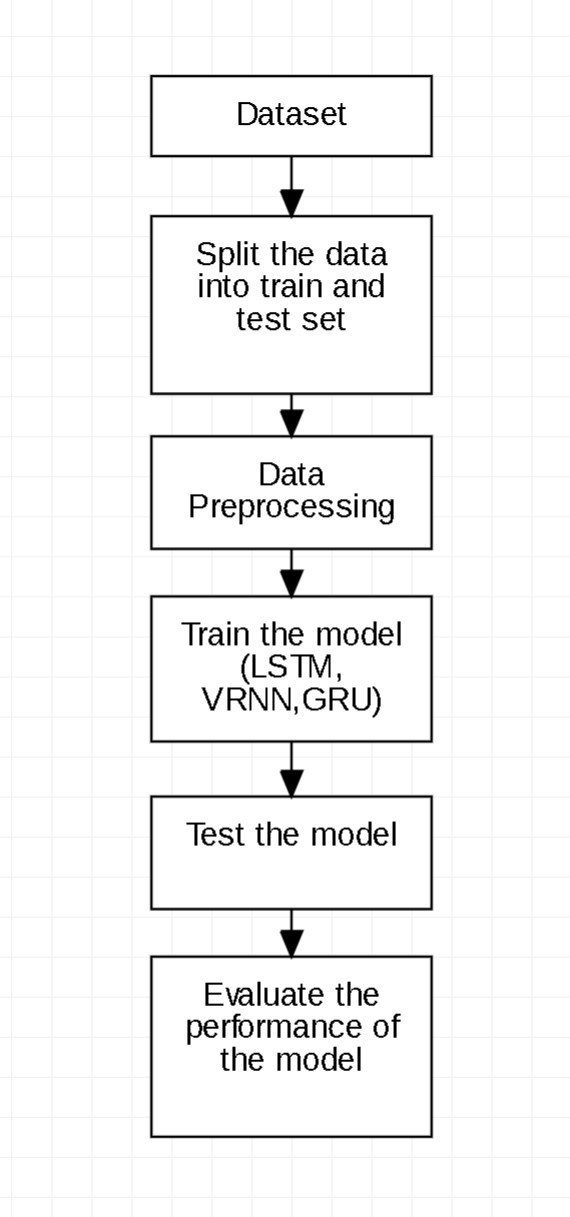
\includegraphics[width=3in]{images/fc.jpg} 
	\caption{Working mechanism of Stock Price Prediction System} %figure name
	\label{Working mechanism of Stock Price Prediction System} % for referencing
\end{center}
\end{figure}
\subsection{Data set}
\vspace{-18pt}
The data set contains financial data, macroeconomic data and technical indicators. Fundamental data is significant or historical data that provides important information needed for stock trading. It has an opening price, closing price, high price, low price and volume. The opening price is the first trading price at the opening of the trading day and the closing price is the last trading price of the stock that day. Likewise, the high and low prices are the highest and lowest prices for that day. Volume refers to the number of products traded in a trading day and indicates traders' interest in the market.High volume means more satisfaction and repetition. All business history data is daily data entry from Share Sansar portal, is one of the popular products providing detailed information about Nepal stock market.
\par
Macroeconomic data is a macroeconomic variable that affects stock market performance. Under the umbrella of macroeconomic factors, the representative features that affect stock price forecasts are remittances (RMT), inflation rate (IR), commercial bank interest rates (CBIR), treasury bills (TRB), consumer price index (CPI) and exchange rate (ER). Remittance is the money Nepalese workers send from abroad. Inflation is the rate of increase in prices over a given period of time.  The commercial bank interest rate is the bank rate at which Nepal Rastra Bank lends money to domestic financial institutions. The treasury bill is typically a promissory maturity note issued by a government as a primary instrument for regulating money supply and raising funds via open market operations. The Consumer Price Index is a measure of the average change overtime in the prices paid by urban consumers for a market basket of consumer goods and services. Exchange rate is the value of one country's currency against another country's currency.
 \par 
Technical indicator includes Moving Average Convergence Divergence (MACD), Average True Range (ATR), Relative Strength Index (RSI), and Money Flow Index (MFI). MACD is calculated by subtracting the 26-day exponential moving average (EMA) from the 12-day EMA. ATR measures the market volatility and is defined as follows:\newpage
\begin{figure}[tbh] % tbh means top, bottom or here (priority: left to right)
\begin{center}
	%
\includegraphics[width = 3in]{images/logo.png}
	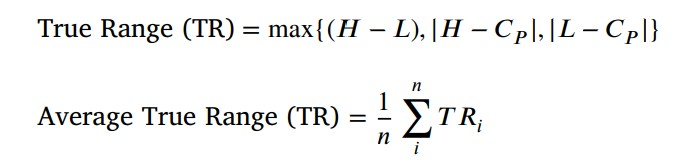
\includegraphics[width=3in]{images/fmla1.jpg} 
	\caption{ATR} %figure name
	\label{ATR} % for referencing
\end{center}
\end{figure}
where, H, L,$ C_p$ represent current high, current low, previous close prices and $T Ri, n$ represent a particular true range, the time period respectively.
\par 
The RSI is a momentum indicator that signals whether a security is overbought or oversold with current price levels, which is computed as follows:\par 
\begin{figure}[tbh] % tbh means top, bottom or here (priority: left to right)
\begin{center}
	%
\includegraphics[width = 3in]{images/logo.png}
	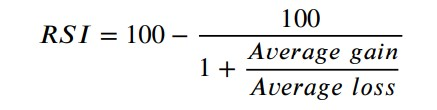
\includegraphics[width=3in]{images/fmla2.jpg} 
	\caption{RSI} %figure name
	\label{RSI} % for referencing
\end{center}
\end{figure}
where average gain and average loss are the average percentage gain and loss calculated over the certain look-back period.
\par 
The MFI communicates a possible reversal in time and provides a signal for further investment. Its calculation starts by finding the typical price (TP), the average of high, low, and close prices for each trading day. If the current TP is higher than the previous one, then positive money flow is calculated by multiplying the current TP with its volume. Similarly, a negative money flow is obtained if the current typical price is lower than the previous one. If the TP does not change, both positive and negative money flow will be zero. Summing all positive money flow indexes leads to positive money flow for a particular period. Negative money flow is calculated similarly. Mathematically, MFI is defined as:
\begin{figure}[tbh] % tbh means top, bottom or here (priority: left to right)
\begin{center}
	%
\includegraphics[width = 3in]{images/logo.png}
	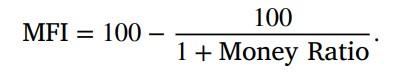
\includegraphics[width=3in]{images/fmla3.jpg} 
	\caption{MFI} %figure name
	\label{MFI} % for referencing
\end{center}
\end{figure}
\subsection{Add dummy variables}
\vspace{-18pt}
The parameters in the data set like addresses are string values but the multiple linear regression can only accept numerical values so they are need to be converted into numerical values. In order to convert it we need to give them the value 0 and 1 on the basis that they are available but there may arise dummy trap problem (when two independent parameters affect each other which can cause conflict in multiple linear regression). So to solve this problem the dummy variables should be one less than the n number of string valued parameters.
\subsection{Filter the data set}
\vspace{-18pt}
All the parameters in the raw data set are not needed for multiple linear regression as some of the parameters have little or no significance in changing the price of the house. So to filter out the useless parameters, we find the single correlation between price of the house and the parameters. Correlation coefficients are used to measure the strength of the linear relationship between two variables. A correlation coefficient greater than zero indicates a positive relationship while a value less than zero signifies a negative relationship.If the correlation is very low or near to zero, they can be neglected.\\
Mathematical calculation for correlation
\begin{equation}
(r_{xy}) =\frac {(n\sum{xy}-\sum{x}\sum{y})}{(\sqrt{[n\sum{x^2}-(\sum{x})^2][n\sum{y^2}-(\sum{y})^2]}}
\end{equation}
\subsection{Split the data set into train set and test set}
\vspace{-18pt}
The data set is divided in train set and test set so that the train set can be used for training the model.
\subsection{Statistical Calculations}
\vspace{-18pt}
For the multiple linear regression, we need to find the values for $\sum{x},\sum{xy},...\sum{x_{n}}$ etc. which are calculated in this stage.
\subsection{Representing the normal equation of multiple linear regression in matrix form}
\vspace{-18pt}
The equation of plane is
\begin{equation}
x=w_{0}+w_{1}x_{1}+w_{2}x_{2}+.....w_{N}x_{N}
\end{equation}
Here,$ x_{1},x_{2},....x_{N}$ are independent parameter variables and x is dependent parameter variable. The intercept is $w_{0}$ and coefficients are $w_{1},w_{2},....w_{N}$.\\
Now to find the values of $w_{0},w_{1},w_{2},...w_{N}$, we need the normal equations which are as follows:
\begin{eqnarray}
\sum{x}= nw_{0}+w_{1}\sum{x_{1}}+w_{2}\sum{x_{2}}+.....w_{N}\sum{x_{N}}\\
\sum{x x_{1}}= w_{0}\sum{x_{1}}+w_{1}\sum{x_{1}}^2+w_{2}\sum{x_{1}x_{2}}+.....w_{N}\sum{x_{1}x_{N}}\\
\sum{x x_{2}}= w_{0}\sum{x_{2}}+w_{1}\sum{x_{1}x_{2}}+w_{2}\sum{x_{2}}^2+.....w_{N}\sum{x_{2}x_{N}}
\end{eqnarray}
\begin{center}
:
\end{center}
\begin{equation}
\sum{x x_{N}}= w_{0}\sum{x_{N}}+w_{1}\sum{x_{1}x_{N}}+w_{2}\sum{x_{2}x_{N}}+.....w_{N}\sum{x_{N}}^2
\end{equation}
Python does not recognize equations so we need to represent these equations in matrix form for further calculations.
\subsection{ Calculation of intercept and coefficients using Gauss Elimination}
\vspace{-18pt}
To find the values of $w_{0},w_{1},w_{2},...w_{N}$, we need to solve the matrices. For this we use the Gauss Elimination method.\\
Algorithm:
\vspace{-18pt}
\begin{enumerate}
\item Start
\item Declare the variables and read the order of the matrix N
\item Take the coefficients of the linear equations as:\\
Do for k= 1 to n\\
Do for j = 1 to n+1\\
Read a[k][j]\\
End for j\\
End for k
\item Do for k= 1 to n-1\\
Do for i= k+1 to n\\
Do for j= k+1 to n+1\\
a[i][j] = a[i][j] -a[i][k]/a[k][k]*a[k][j]\\
End for j\\
End for i\\
End for k
\item Compute x[n] = a[n][n+1]/a[n][n]
\item Do for k= n-1 to 1\\
sum = 0\\
Do for j = k+1 to n\\
sum += a[k][j]*x[j]\\
End for j\\
x[k] = 1/a[k][k] * (a[k][n+1] - sum)\\
End for k
\item Display the result x[k]
\item Stop 
\end{enumerate}
\subsection{Calculation and Evaluation of predicted price}
\vspace{-18pt}
Now the calculated values of intercept and coefficients are inserted in the equation (3.2) to calculate the predicted price.\\
We evaluated model’s performance using metrics: the coefficient of determination $R^2$, Root Mean Squared Error(RMSE).\\
RMSE: It can be defined as the standard sample deviation between the predicted values and the observed ones. It is to be noted that unit of RMSE is same as dependent variable y .The lower RMSE values are indicative of a better fit model. If the model's primary objective is prediction then RMSE is a stronger measure.\\
R-squared: The R-square value provides a measure of how much the model replicates the actual results, based on the ratio of total variation of outcomes as explained in the model.The higher the R-squared, the better the model fits the data given. The R-squared value ranges from 0 to 1, representing the percentage of a squared correlation between the target variable's expected and real values. But in case of multiple linear regressions, R-squared value may increase with increasing features even though the model is not actually improving. A related, Adjusted R-squared statistic can be used to address this disadvantage. This measures the model's goodness and penalizes the model to use more predictors.
\section{System Diagram}
\vspace{-18pt}
\subsection{Use case diagram}
\newpage 
\begin{figure}
	%
\includegraphics[width = 3in]{images/logo.png}
	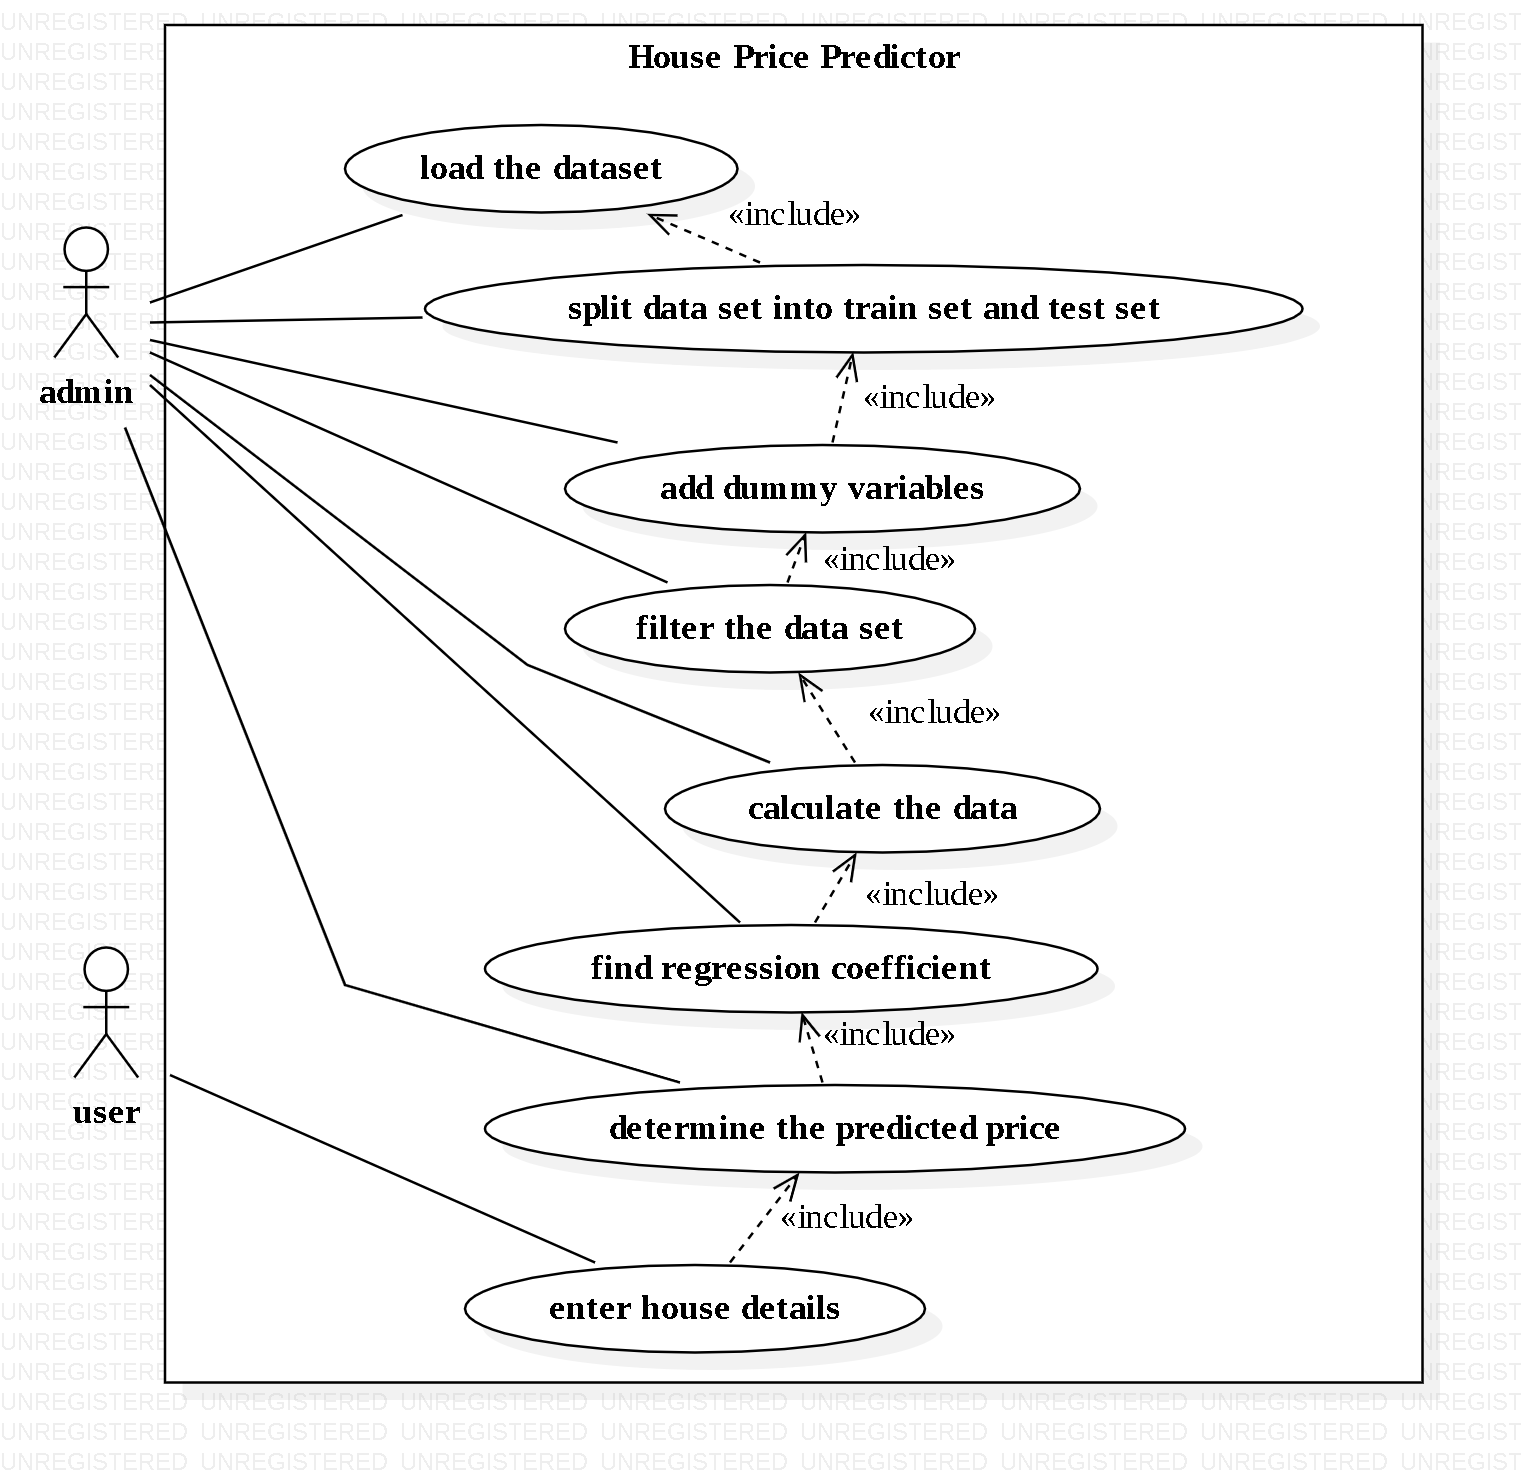
\includegraphics[width=6in]{UseCaseDiagram1.png} 
	\caption{Use case Diagram of House Price Prediction System} %figure name
	\label{Use case Diagram of House Price Prediction System} % for referencing
\end{figure}
\newpage
 \subsection{DFD level diagram}
\begin{figure}
\begin{center}
	%
\includegraphics[width = 3in]{images/logo.png}
	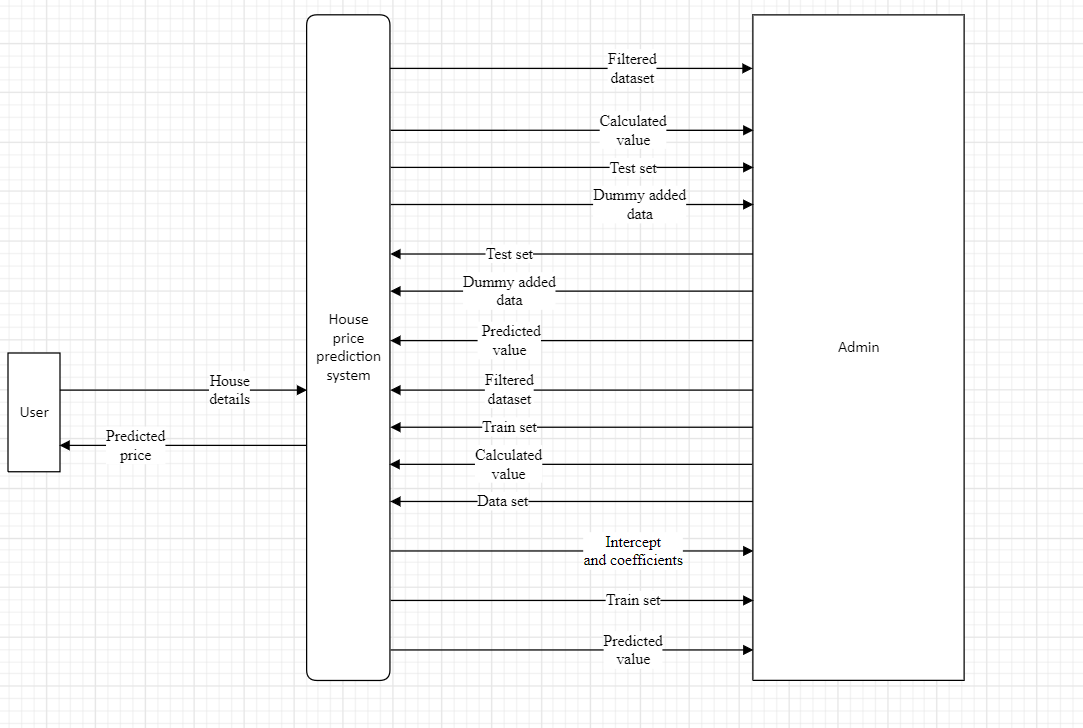
\includegraphics[width=5in]{dfd0.png} 
	\caption{DFD Level 0 diagram of House Price Prediction System} %figure name
	\label{DFD Level 0 diagram of House Price Prediction System} % for referencing
\end{center}
\end{figure}
\begin{figure}
\begin{center}
	%
\includegraphics[width = 3in]{images/logo.png}
	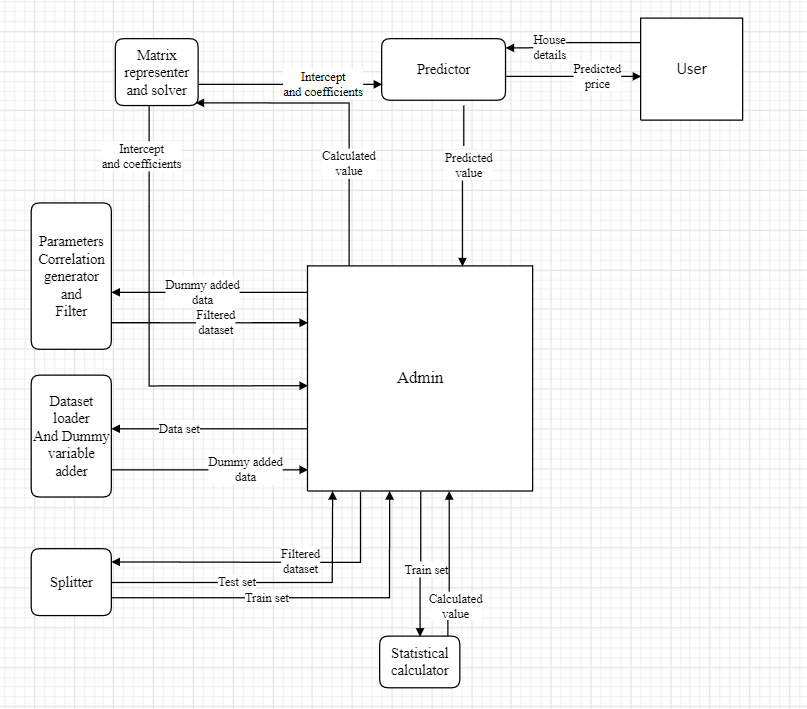
\includegraphics[width=5in]{dfd12.png} 
	\caption{DFD Level 1 diagram of House Price Prediction System} %figure name
	\label{DFD Level 1 diagram of House Price Prediction system} % for referencing
\end{center}
\end{figure}
\newpage
\subsection{Software Development Model}
 \begin{figure}[tbh] % tbh means top, bottom or here (priority: left to right)
\begin{center}
	%
\includegraphics[width = 3in]{images/logo.png}
	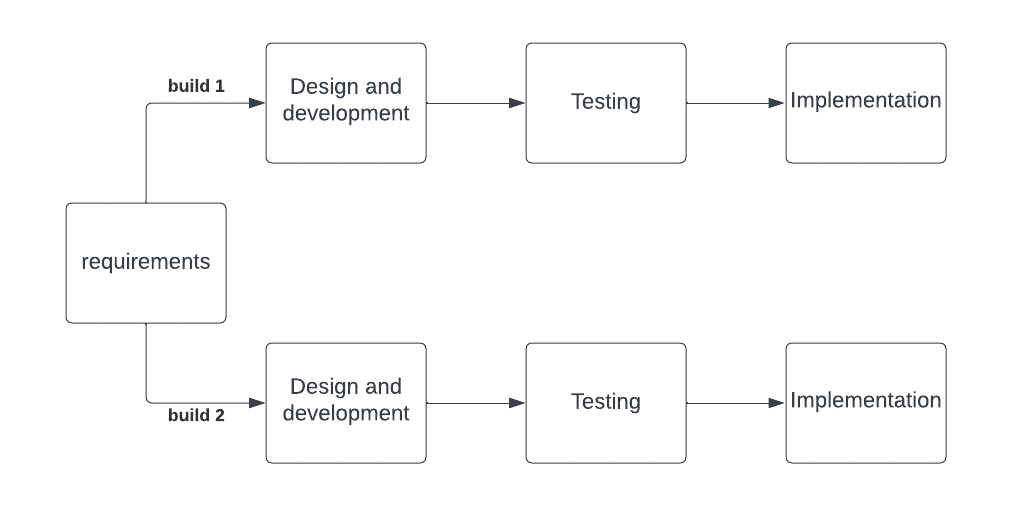
\includegraphics[scale=1]{incre.png} 
	\caption{Incremental Model} %figure name
	\label{Incremental Model} % for referencing
\end{center}
\end{figure}
 Incremental model is a method of software engineering that combines the elements of waterfall model in iterative manner. It involves both development and maintenance. In this model requirements are broken down into multiple modules. Incremental development is done in steps from analysis design, implementation, testing/verification, maintenance. Each iteration passes through the requirements, design, coding and testing phases. The first increment is often a core product where the necessary requirements are addressed, and the extra features are added in the next increments. The core product is delivered to the client. Once the core product is analyzed by the client, there is plan development for the next increment.\\
\chapter{Results and Discussion}
\section{Result}
\vspace{-18pt}
We have completed the design and development of the project along with obtaining the desired output of the project. The project currently takes in location, area(square feet), bhk and balcony and predicts the price of the house through linear regression. The interface of the project is shown below: \par
\begin{figure}[tbh] % tbh means top, bottom or here (priority: left to right)
\begin{center}
	%
\includegraphics[width = 3in]{images/logo.png}
	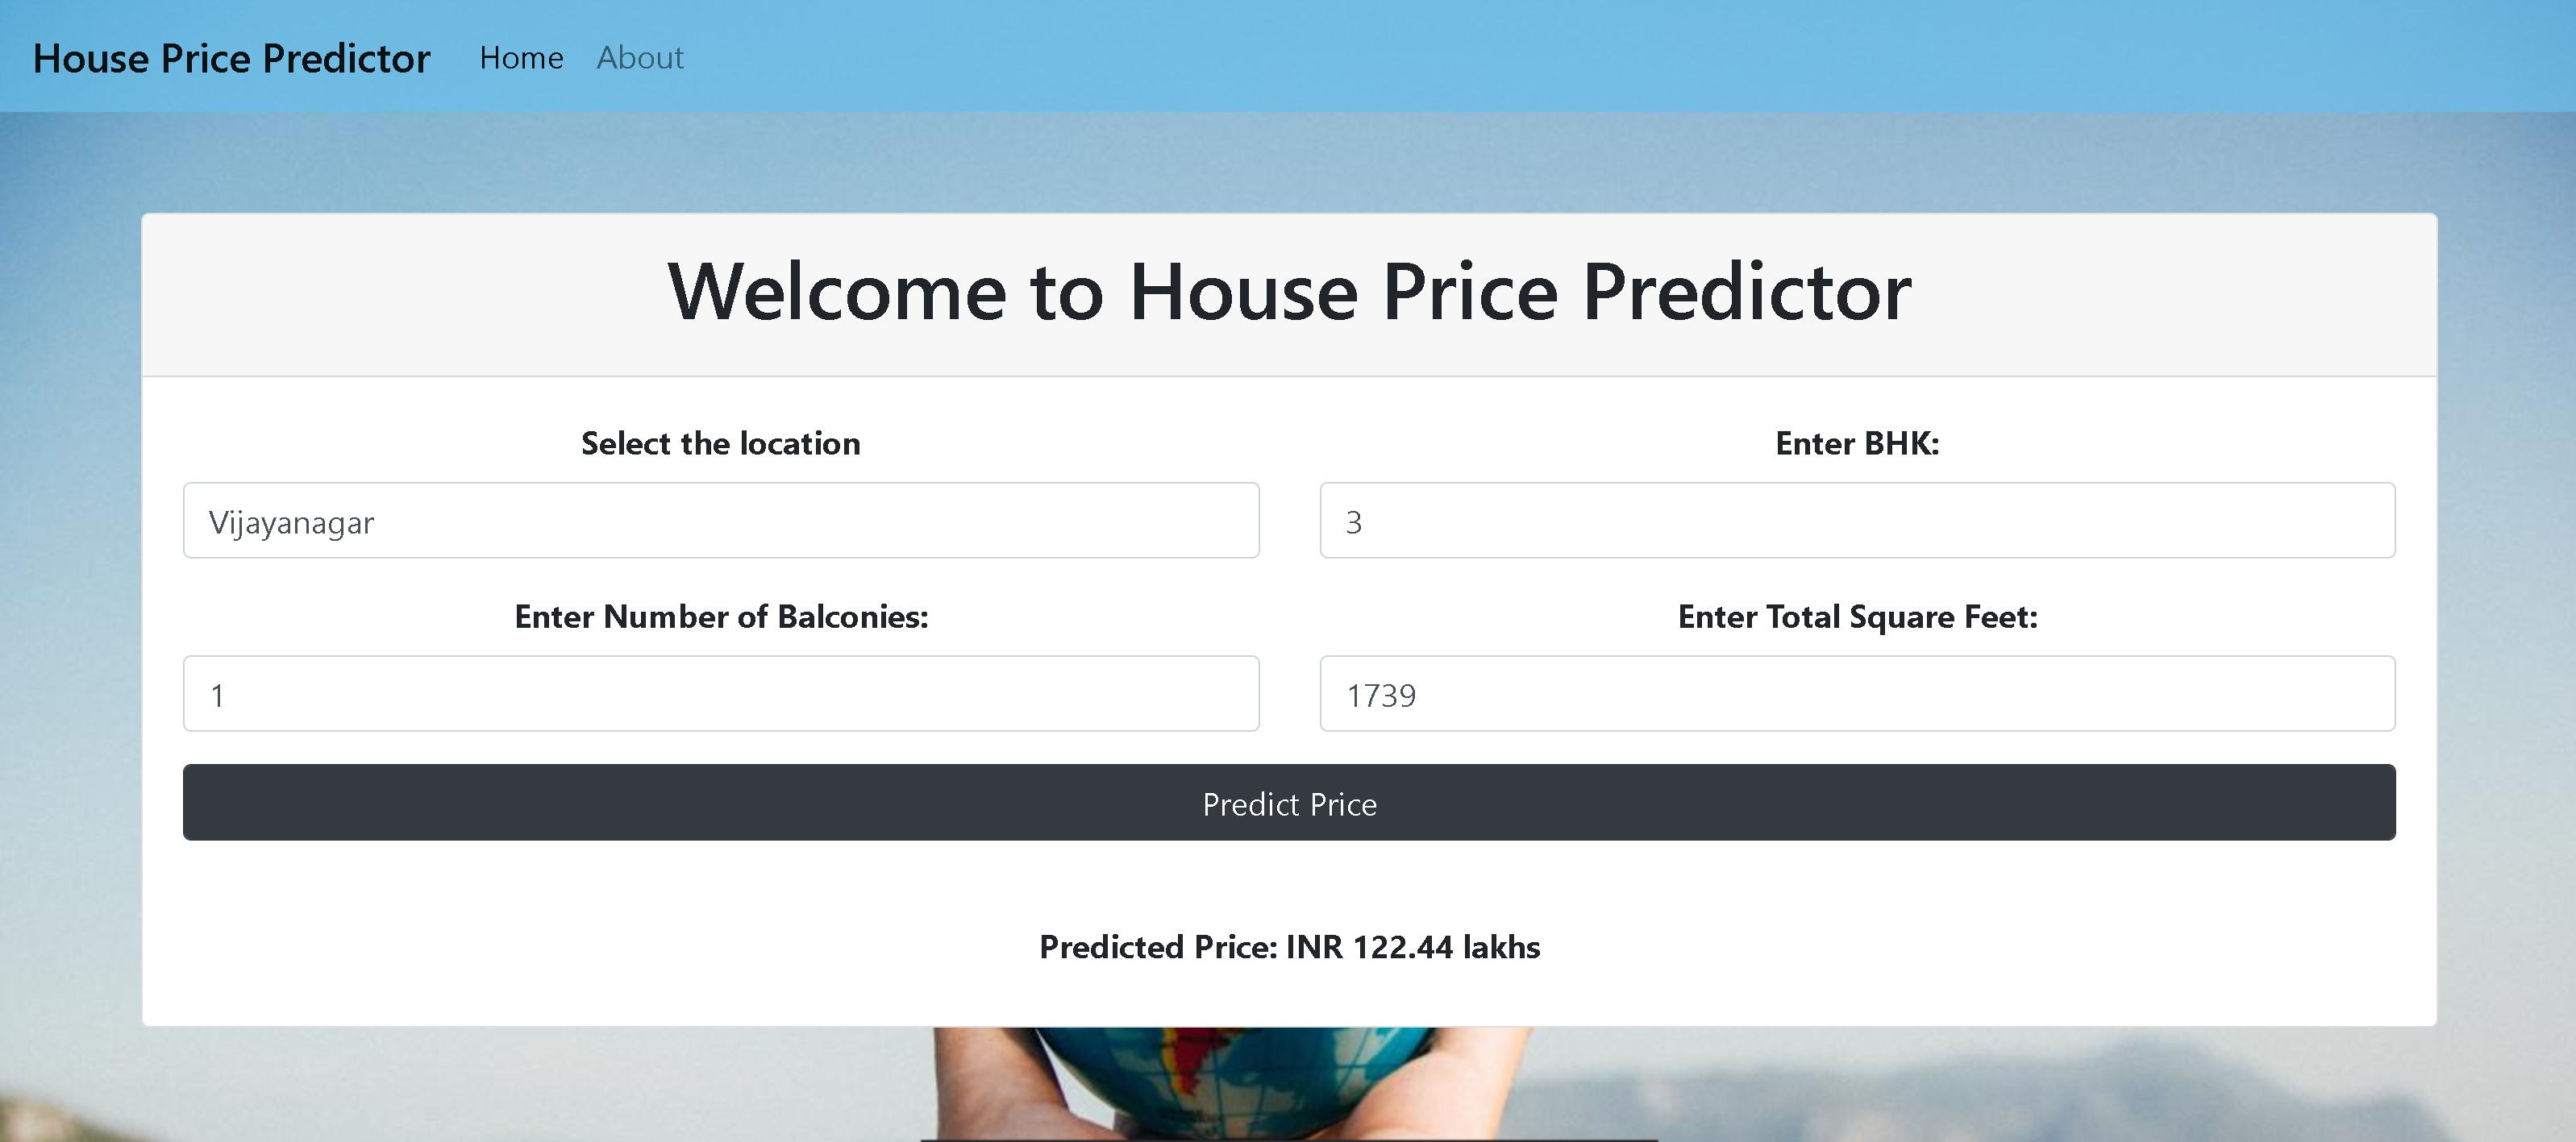
\includegraphics[width=5in]{hh1.jpg} 
	\caption{Home Page} %figure name
	\label{Home Page} % for referencing
\end{center}
\end{figure}
\begin{figure}[tbh] % tbh means top, bottom or here (priority: left to right)
\begin{center}
	%
\includegraphics[width = 3in]{images/logo.png}
	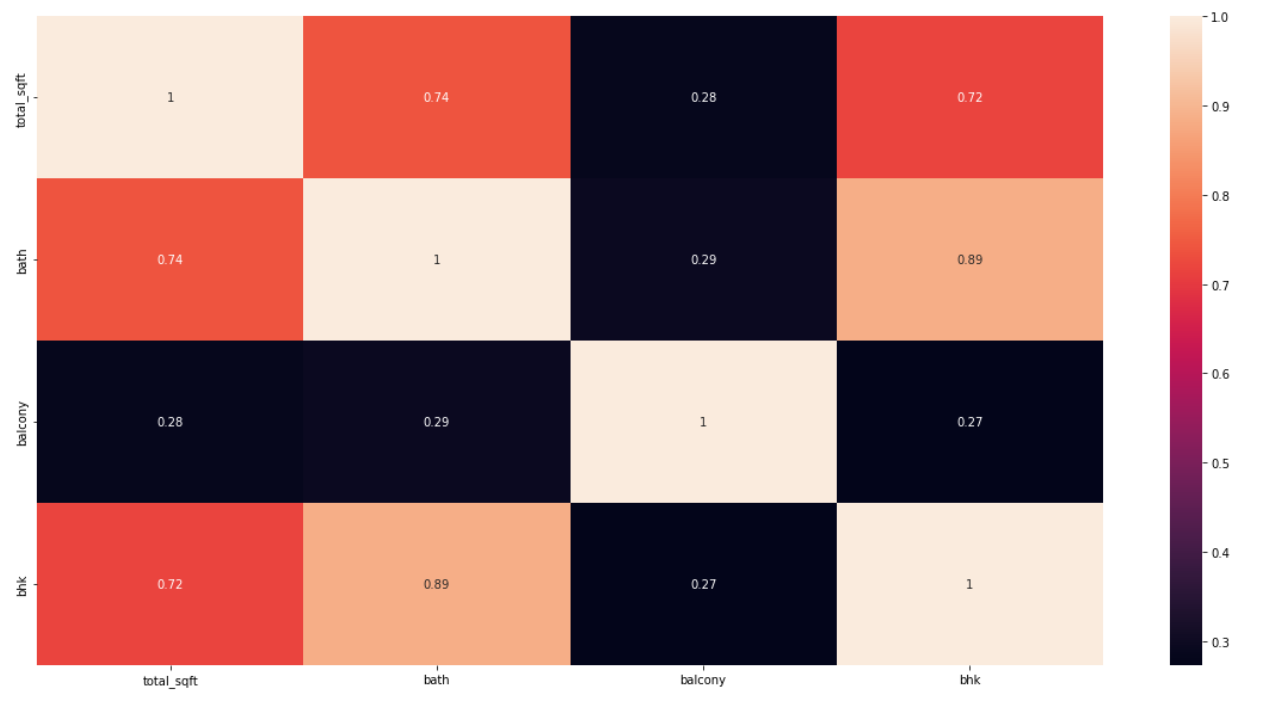
\includegraphics[width=5in]{heatmap.png} 
	\caption{Heat map for correlation } %figure name
	\label{Heat map for correlation} % for referencing
\end{center}
\end{figure}
From Figure 4.2, we can see that the correlation between bathroom and bhk is very high so we can ignore one of them. In our case, we have ignored bathroom.
\newpage
\begin{figure} % tbh means top, bottom or here (priority: left to right)
\begin{center}
	%
\includegraphics[width = 3in]{images/logo.png}
	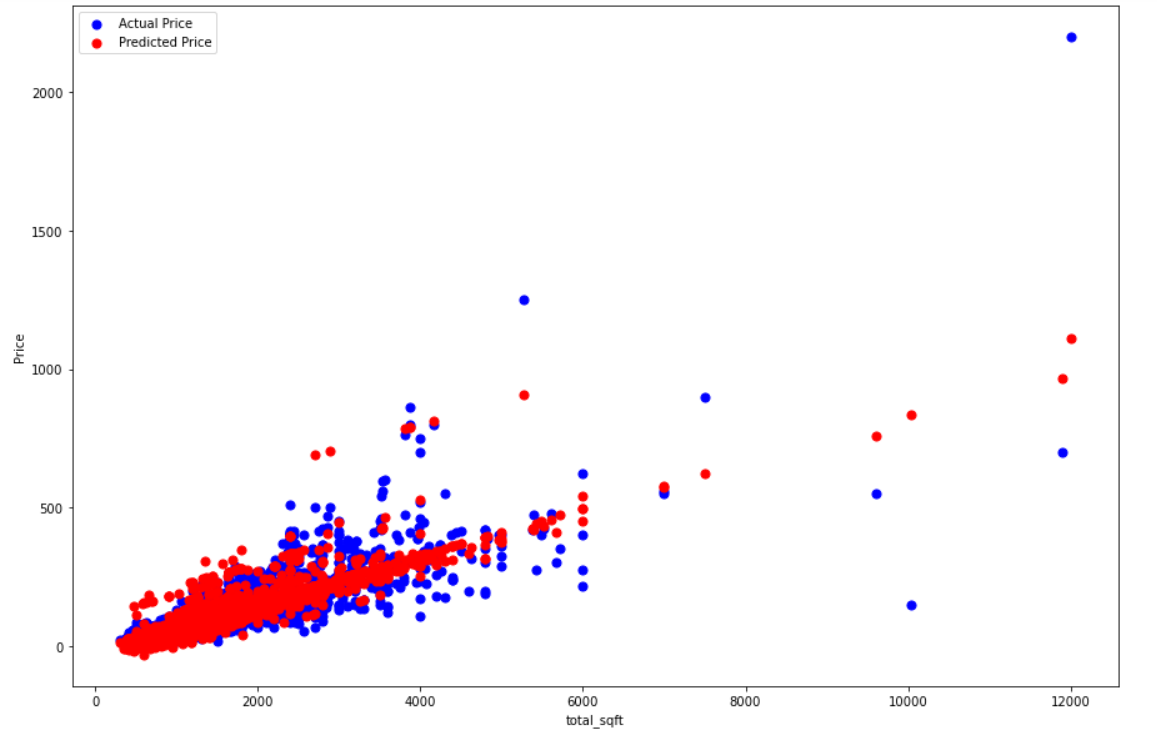
\includegraphics[width=6in]{scplot.png} 
	\caption{Scatter plot } %figure name
	\label{Scatter plot} % for referencing
\end{center}
\end{figure}
From the above figure, it can be concluded that for some data points, the actual price is very close to the predicted price which means that for some data points the model is highly accurate. However, the figure also shows that for some points the difference between the actual price and the predicted price is large which shows that for some data 
points the result is less accurate. Overall, we can say that the model has a decent amount of accuracy.
\begin{figure}[tbh] % tbh means top, bottom or here (priority: left to right)
\begin{center}
	%
\includegraphics[width = 3in]{images/logo.png}
	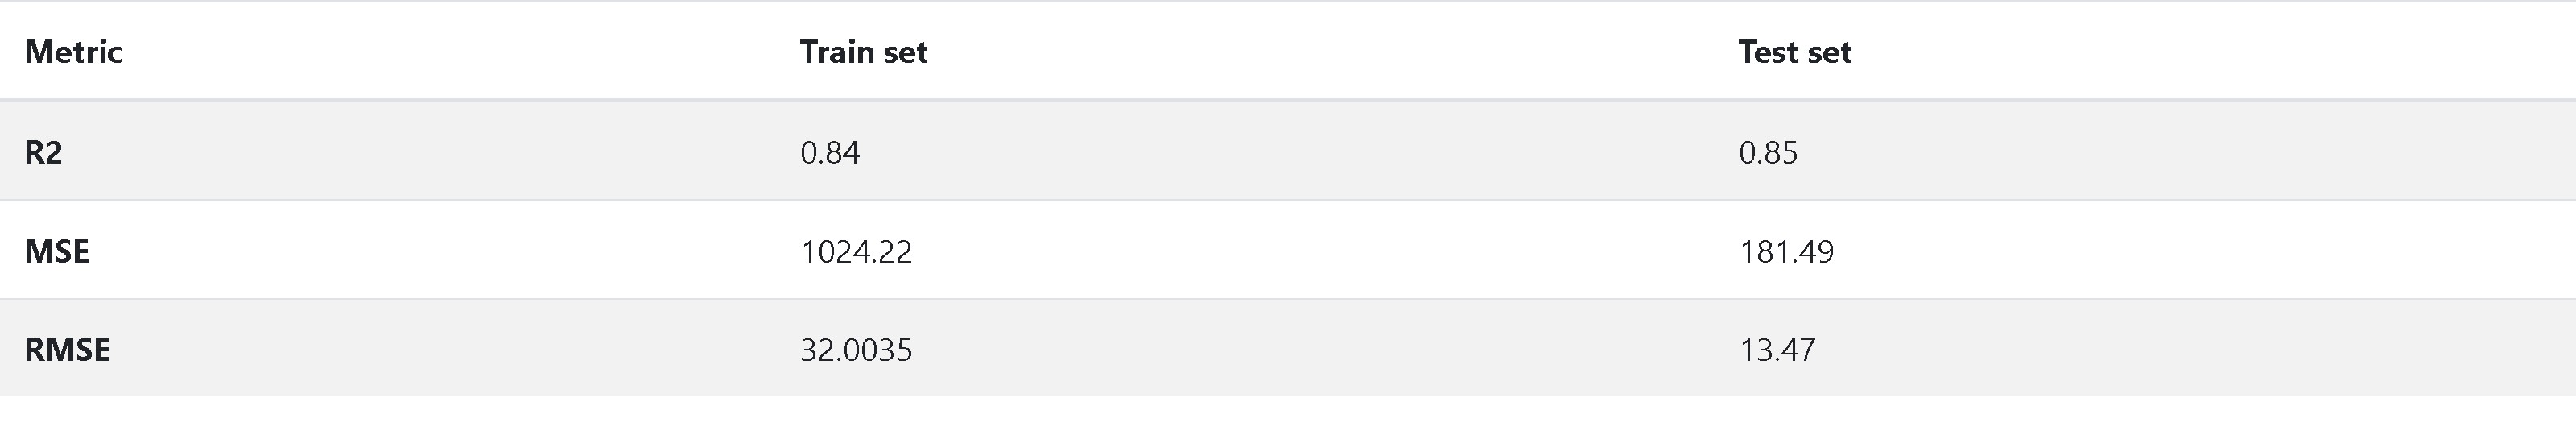
\includegraphics[width=6in]{ww.jpg} 
	\caption{Evaluation metrics } %figure name
	\label{Evaluation metrics} % for referencing
\end{center}
\end{figure}
%\newpage
\section{Discussion}
\vspace{-18pt}
House Price Predictor system is a website that predicts the prices of houses based on location, area, number of balconies and bhk. For front end development of the website, we have used HTML,CSS and JS. We used Pandas and numpy libraries for accessing dataframe. Matplotlib is used for data visualisation. We have done predictions with the help of Linear Regression, Correlation and Gauss Elimination method. Evaluation of the system was done by R-squared, Mean Squared Error and Root Mean Squared Error. Flask framework was used to connect the front end and back end of our website. 
\section{Limitations}
\vspace{-18pt}
\begin{enumerate}
\item  Outliers can have huge effects on the regression.
\item Linear Regression also looks at a relationship between the mean of the dependent variables and the independent variables. Just as the mean is not a complete description of a single variable, linear regression is not a complete description of relationships among variables.
\end{enumerate} 
\chapter{Conclusion and Future Enhancements}
\vspace{-18pt}
\section{Conclusion}
\vspace{-18pt}
In this project, we have used the regression model to predict the price of different houses. It comes under the area of supervised learning which is one of the types of machine learning. All the steps required for the successful completion of the house price prediction system have been completed.
\section{Future Enhancements}
\vspace{-18pt}
\begin{enumerate}
\item increase and update the data set on a regular basis
\item add locations for Nepal
\end{enumerate}
%\chapter*{References}
%Reference
\renewcommand\bibname{References} % Change heading to References
\bibliographystyle{IEEEtr} % to use IEEE Format for referencing
\addcontentsline{toc}{chapter}{References} % to add references in TOC
\bibliography{library} % specify the .bib file containing reference information 
\end{document}
